\section{Experimental design and attribution protocol}
\label{sec:validation}

The experiments answer three different questions: whether a discretization reaches the prescribed physical accuracy, whether an implementation preserves that discretization, and whether a qualified implementation reduces complete solution time. These questions require different controls. A successful trajectory is evidence for numerical feasibility; a fast isolated operator is evidence about that operator; a complete paired timing campaign is required to establish a practical speed advantage. We retain these distinctions when reporting both successful and unsuccessful candidates.

\subsection{Problem, references, and independent reconstruction}

All main comparisons concern the finite annulus with $a=0.5$, $R=6$, $\nu=0.01$, and $T=72$. The final incident speed and cylinder diameter are both unity, giving $\mathrm{Re}=100$. The transverse pulse ends at $t=12$, whereas the observations extend to $t=72$. No reflection constraint is imposed, and neither the fields nor the probe series are shifted in time or aligned by wake phase. This is necessary because accumulated phase error is part of the approximation error for an initial-boundary-value problem.

The two frozen numerical references, denoted \texttt{angular\_fine} and \texttt{time\_fine} in the archive, resolve angular and temporal refinement separately within a finite-difference refinement chain. The chain increases the radial resolution from 384 to 448 intervals, angular truncation from 128 to 144, and step rate from 384 to 512. They are distinct numerical references, not two independently implemented continuum-solution certificates. Their combined late-time discrepancy is $0.0290144\%$. This is below the empirical reference allowance of $0.125\%$, one quarter of the candidate tolerance. It is above the $0.025\%$ allowance that the same rule would assign to a $0.1\%$ candidate tolerance. Consequently the current reference evidence supports the reported $0.5\%$ protocol, without establishing a certified continuum error or a tighter accuracy target.

Evaluation is performed after reconstructing every method on the same physical grids. For reconstruction grid $G$, checkpoint $t$, and its physical weights, define
\begin{equation}
\label{eq:field-errors}
 E_u(G,t)=\frac{\|\boldsymbol u-\boldsymbol u_{\rm ref}\|_G}{\|\boldsymbol u_{\rm ref}\|_G},\qquad
 E_\omega(G,t)=\frac{\|\omega-\omega_{\rm ref}\|_G}{\|\omega_{\rm ref}\|_G}.
\end{equation}
The measure is $r^2\,ds\,d\theta$, and the velocity norm combines both polar components. Each quantity is checked over the full annulus and over $r\leq2.5$. The reconstruction grids use 123, 129, and 144 radial points and respectively 433, 449, and 457 shifted angular points. They differ from the solver quadrature and FFT grids. Their construction and the 19 physical checkpoint times are listed in Appendix~\ref{sec:app-setup}. Taking the maximum across grids reduces dependence on an individual sampling pattern, but remains a finite set of discrete tests.

There are 19 reference-scored physical checkpoints from $t=0.5$ to $72$. A piecewise schedule saves two additional states immediately after the bridge for implementation comparison; the archive therefore distinguishes 19 physical checkpoints from 21 saved implementation checkpoints. Six probe histories, transverse velocity and vorticity at three downstream positions, contain 577 equally spaced times, including the zero initial value. The implementation tolerance against the CPU trajectory of the same discretization is $10^{-5}$ for the field and complete probe-series comparisons. The wake checker additionally verifies sustained alternating signs. Neither a plausible shedding frequency nor a visually similar wake substitutes for the field-error tests.

\subsection{A safeguard against compensating errors}

For a piecewise schedule, the constant-step control uses the same space, seed, geometry, and quadrature. Let $v$ be this control, $w$ the piecewise candidate, and $z$ a reference, all evaluated in the same weighted norm. Define $b=\|v-z\|_G/\|z\|_G$ and $d=\|w-v\|_G/\|v\|_G$. Then
\begin{equation}
\label{eq:triangle-guard}
 \frac{\|w-z\|_G}{\|z\|_G}
 \leq b+d\frac{\|v\|_G}{\|z\|_G}
 \leq b+(1+b)d.
\end{equation}
Both the direct error and $b+(1+b)d$ must be at most $0.005$. Using $b+d$ would incorrectly ignore the different denominators. The bound is evaluated for each prescribed field, region, grid, checkpoint, and reference, before taking maxima. It prevents a candidate from qualifying solely because the schedule error cancels part of its constant-step error. It is a rigorous relation between these discrete fields, not an a posteriori bound against the exact PDE solution.

This extra test can reject a candidate whose direct error passes. For high-resolution Legendre34, the piecewise direct field score is approximately $0.481690\%$, but the triangle safeguard is $0.509600\%$. Its constant-step variant remains eligible. Keeping that cheaper deterministic alternative is essential: applying a common accuracy target does not require every method to use an identical schedule when the question is minimum cost at that target.

\subsection{Controlled comparisons and computational environment}

Table~\ref{tab:fairness} separates the effects being compared. A same-rank comparison controls algebraic dimension but does not prove equal approximation power for all flows. A comparison of the least expensive qualifying configurations instead permits different ranks and schedules. Both are useful, and their conclusions must be labeled accordingly. The finite-difference baseline uses fourth-order radial spatial differences and the same second-order SBDF2 time family; ``fourth order'' does not describe its time discretization.

\begin{table}[tbp]
\centering\small
\caption{Comparison matrix and the effect each contrast can identify. All physical comparisons retain the same boundary-value problem and error criteria.}
\label{tab:fairness}
\begin{tabularx}{\linewidth}{@{}p{0.21\linewidth}XX@{}}
\toprule
Contrast & Held fixed & Quantity allowed to change \\
\midrule
RFM / Legendre at equal rank & $K,q$, retained rank, schedule, shared kernels and runtime policy & Trial functions and resulting approximation error \\
Accuracy-matched spaces & Reference, field and probe tests, runtime policy & Rank and qualified schedule; actual rank reported per seed \\
Constant / piecewise & Same trial space, seed, $K,q$ and observation protocol & Step schedule and associated phase preparation \\
cuFFT / fused operator & Input state, precision, retained spectrum, normalization and output definition & Transform implementation and temporary storage \\
Serial / warp observation & State evolution and probe weights & Floating-point summation order and observation cost \\
First use / cache hit & Solver, artifacts, accuracy criteria and fresh-process entry & Explicit compilation-artifact availability \\
Galerkin / FD & Physical problem, accuracy target, observation and runtime policies & Spatial discretization and its qualified resolution \\
\bottomrule
\end{tabularx}
\end{table}

The recorded experimental machine and software are summarized in Table~\ref{tab:hardware}. The numerical backend uses FP64 CUDA kernels and cuFFT through a native interface. The CPU reference and host preparation use NumPy and SciPy. A compatibility probe also exercised cuBLAS, but the native Galerkin march uses project-specific projection kernels; cuBLAS should not be credited as the production projection backend.

\begin{table}[tbp]
\centering\small
\caption{Recorded environment of the archived Windows experiments. Version labels describe the measured environment, not a recommendation to use the latest available release.}
\label{tab:hardware}
\begin{tabularx}{\linewidth}{@{}lX@{}}
\toprule
Component & Recorded value \\
\midrule
CPU & AMD Ryzen 9 9955HX, 16 cores, 32 logical processors \\
GPU & NVIDIA GeForce RTX 5060 Laptop GPU; compute capability 12.0 \\
Operating system / driver & Windows 11, build 26200; NVIDIA 596.13, WDDM \\
Scientific runtime & Python 3.13.5; NumPy 2.2.6; SciPy 1.16.3 \\
Main CUDA components & CUDA 11.8 NVRTC and cuFFT; driver API version 13020 \\
Precision and host threading & FP64 arithmetic; one BLAS thread in controlled comparisons \\
Main observation / nonlinear path & Warp probe reduction / original batched cuFFT \\
\bottomrule
\end{tabularx}
\end{table}

Independent qualification reconstruction can use several CPU workers while a single owner captures GPU trajectories. Those elapsed times are excluded from method rankings. The intended latency experiment instead runs one GPU solve at a time with fixed affinities, an identical runtime policy, and sampled external-load checks. Low total CPU utilization during this experiment is expected: one controlled host core is only one of 32 logical processors. Concurrent throughput is a different objective and was not measured by this campaign.

\section{Accuracy, trial-space size, and nonlinear workload}
\label{sec:accuracy-results}

\subsection{Qualified configurations and retained ranks}

Table~\ref{tab:configurations} lists the main configurations. The RFM and Legendre suffixes denote input basis counts, whereas the retained rank is obtained after enrichment, scaling, and truncation. The mean block retains rank 30 throughout. A finite-difference label $n$ counts radial intervals, giving $n+1$ nodes and $n-1$ interior unknowns per angular mode. These interval counts are not directly comparable to a Galerkin retained rank.

\begin{table}[tbp]
\centering\small
\caption{Spatial configurations and eligible step-rate schedules. An arrow denotes the change at $t=8$.}
\label{tab:configurations}
\begin{tabularx}{\linewidth}{@{}Xcl>{\raggedright\arraybackslash}p{0.27\linewidth}@{}}
\toprule
Configuration & Rank & $K/q$ & Step rate \\
\midrule
Mid RFM37 & 39 & $72/66$ & $128$ or $128\to112$ \\
Mid Legendre35 & 39 & $72/66$ & $128$ or $128\to112$ \\
High RFM41 & 40 & $80/76$ & $152$ or $152\to136$ \\
High RFM35 & 38 or 39 & $80/76$ & $152$ or $152\to136$ \\
High Legendre36 / 35 & 40 / 39 & $80/76$ & $152$ or $152\to136$ \\
High Legendre34 & 38 & $80/76$ & $152$ only \\
FD176 dense / FD184 banded & --- & $K=80$ & $128$ throughout \\
\bottomrule
\end{tabularx}
\end{table}

There are 39 unique numerical identities, each evaluated under two explicit compilation-cache policies, for 78 GPU trajectories through $T=72$. Every trajectory passed the registered physical, implementation, and wake criteria. Within each of the 39 cache-policy pairs, saved states, times, and probe arrays were bitwise identical. These are 39 numerical configurations reproduced under two policies, not 78 independent random-feature samples.

\begin{table}[tbp]
\centering\small
\caption{Worst errors by method and schedule, in percent. Each entry includes all registered seeds, both cache policies, the references, reconstruction grids, and checkpoints. Velocity and vorticity include full-domain and near-field checks.}
\label{tab:accuracy}
\begin{tabularx}{\linewidth}{@{}Xlrrr@{}}
\toprule
Configuration & Schedule & Velocity & Vorticity & Guard \\
\midrule
RFM37 / K72 & Uniform & 0.02943 & 0.40960 & — \\
RFM37 / K72 & Piecewise & 0.04467 & 0.43168 & 0.47865 \\
Leg35 / K72 & Uniform & 0.02676 & 0.44207 & — \\
Leg35 / K72 & Piecewise & 0.04104 & 0.45665 & 0.49773 \\
FD176 / K80 & Uniform & 0.10497 & 0.40876 & — \\
RFM41 / K80 & Uniform & 0.01819 & 0.33189 & — \\
RFM41 / K80 & Piecewise & 0.02595 & 0.34034 & 0.36867 \\
Leg36 / K80 & Uniform & 0.01613 & 0.36205 & — \\
Leg36 / K80 & Piecewise & 0.01972 & 0.36634 & 0.39405 \\
Leg35 / K80 & Uniform & 0.01896 & 0.41520 & — \\
Leg35 / K80 & Piecewise & 0.02235 & 0.41914 & 0.44722 \\
FD184 / K80 & Uniform & 0.07900 & 0.30652 & — \\
RFM35 / K80 & Uniform & 0.01935 & 0.42818 & — \\
RFM35 / K80 & Piecewise & 0.02309 & 0.43245 & 0.46494 \\
Leg34 / K80 & Uniform & 0.02301 & 0.47754 & — \\
\bottomrule
\end{tabularx}

\end{table}

Across the full cohort, the maximum direct physical error is $0.477543\%$, and the maximum safeguard is $0.497730\%$. The latter leaves only approximately $0.002270$ percentage points below the $0.5\%$ limit. It is a measured acceptance margin rather than evidence of robustness to changes in Reynolds number, boundary conditions, or floating-point environment. The largest velocity error across full and near fields is $0.10497\%$; thus the tightest constraints arise from vorticity. This explains why velocity-only validation would have admitted a substantially weaker test.

The largest GPU-to-CPU field error is $3.5721\times10^{-6}$ and the largest probe-series error is $3.8792\times10^{-6}$, both below $10^{-5}$. These maxima correspond to the finite-difference control. For the final rank-expanded cases lacking a historical serial-observer control, the qualification still uses the registered CPU and reference comparisons; an unavailable earlier observer pairing is not silently treated as additional evidence.

\subsection{Seed variation and the deterministic alternative}

The five RFM seeds are fixed before the final qualification: 7331, 7687, 8011, 8353, and 9041. Table~\ref{tab:seeds} exposes a confounding factor that is hidden if only the input label RFM35 is reported. Four seeds retain 38 radial functions and one retains 39. The smaller vorticity error for seed 8353 therefore occurs in a larger retained space. It cannot be attributed solely to a better draw of equal-dimensional features. Five fixed seeds also do not support a probabilistic guarantee over the feature distribution.

\begin{table}[tbp]
\centering\small
\caption{High-resolution RFM35 by seed. Errors and safeguards are percentages, recomputed from the archived qualification scores; the two cache policies give the same arrays.}
\label{tab:seeds}
\begin{tabularx}{\linewidth}{@{}rrXXX@{}}
\toprule
Seed & Rank & Constant-step $E_\omega$ & Piecewise $E_\omega$ & Piecewise safeguard \\
\midrule
7331 & 38 & 0.427183 & 0.431520 & 0.463945 \\
7687 & 38 & 0.427945 & 0.432246 & 0.464707 \\
8011 & 38 & 0.428183 & 0.432451 & 0.464943 \\
8353 & 39 & 0.378031 & 0.383875 & 0.414801 \\
9041 & 38 & 0.427611 & 0.431910 & 0.464372 \\
\bottomrule
\end{tabularx}
\end{table}

The rank-38 Legendre34 constant-step method also qualifies. Thus the evidence supports compact random-feature and deterministic polynomial spaces at this tolerance, but does not establish that randomness is necessary for compactness. A fair cost comparison must retain Legendre34 even though its piecewise variant fails, and must include Legendre35 and Legendre36 to separate equal-rank from accuracy-matched contrasts. High-resolution Legendre33 fails the $T=72$ accuracy tests; a short-horizon pass is insufficient for promotion. The reduced mid-resolution RFM35 screen also does not replace the registered five-seed RFM37 cohort.

\subsection{Wake dynamics and the cost removed by scheduling}

Figures~\ref{fig:annulus-wake} and \ref{fig:wake-probes} show the retained asymmetry and alternating shedding. The images display a local window, while scoring covers the prescribed full and near domains. The probe plot combines qualified trajectories and a fine reference for physical interpretation. Its curves are not from a single isolated timing batch and are not used to estimate errors by inspection.

\begin{figure}[tbp]
\centering
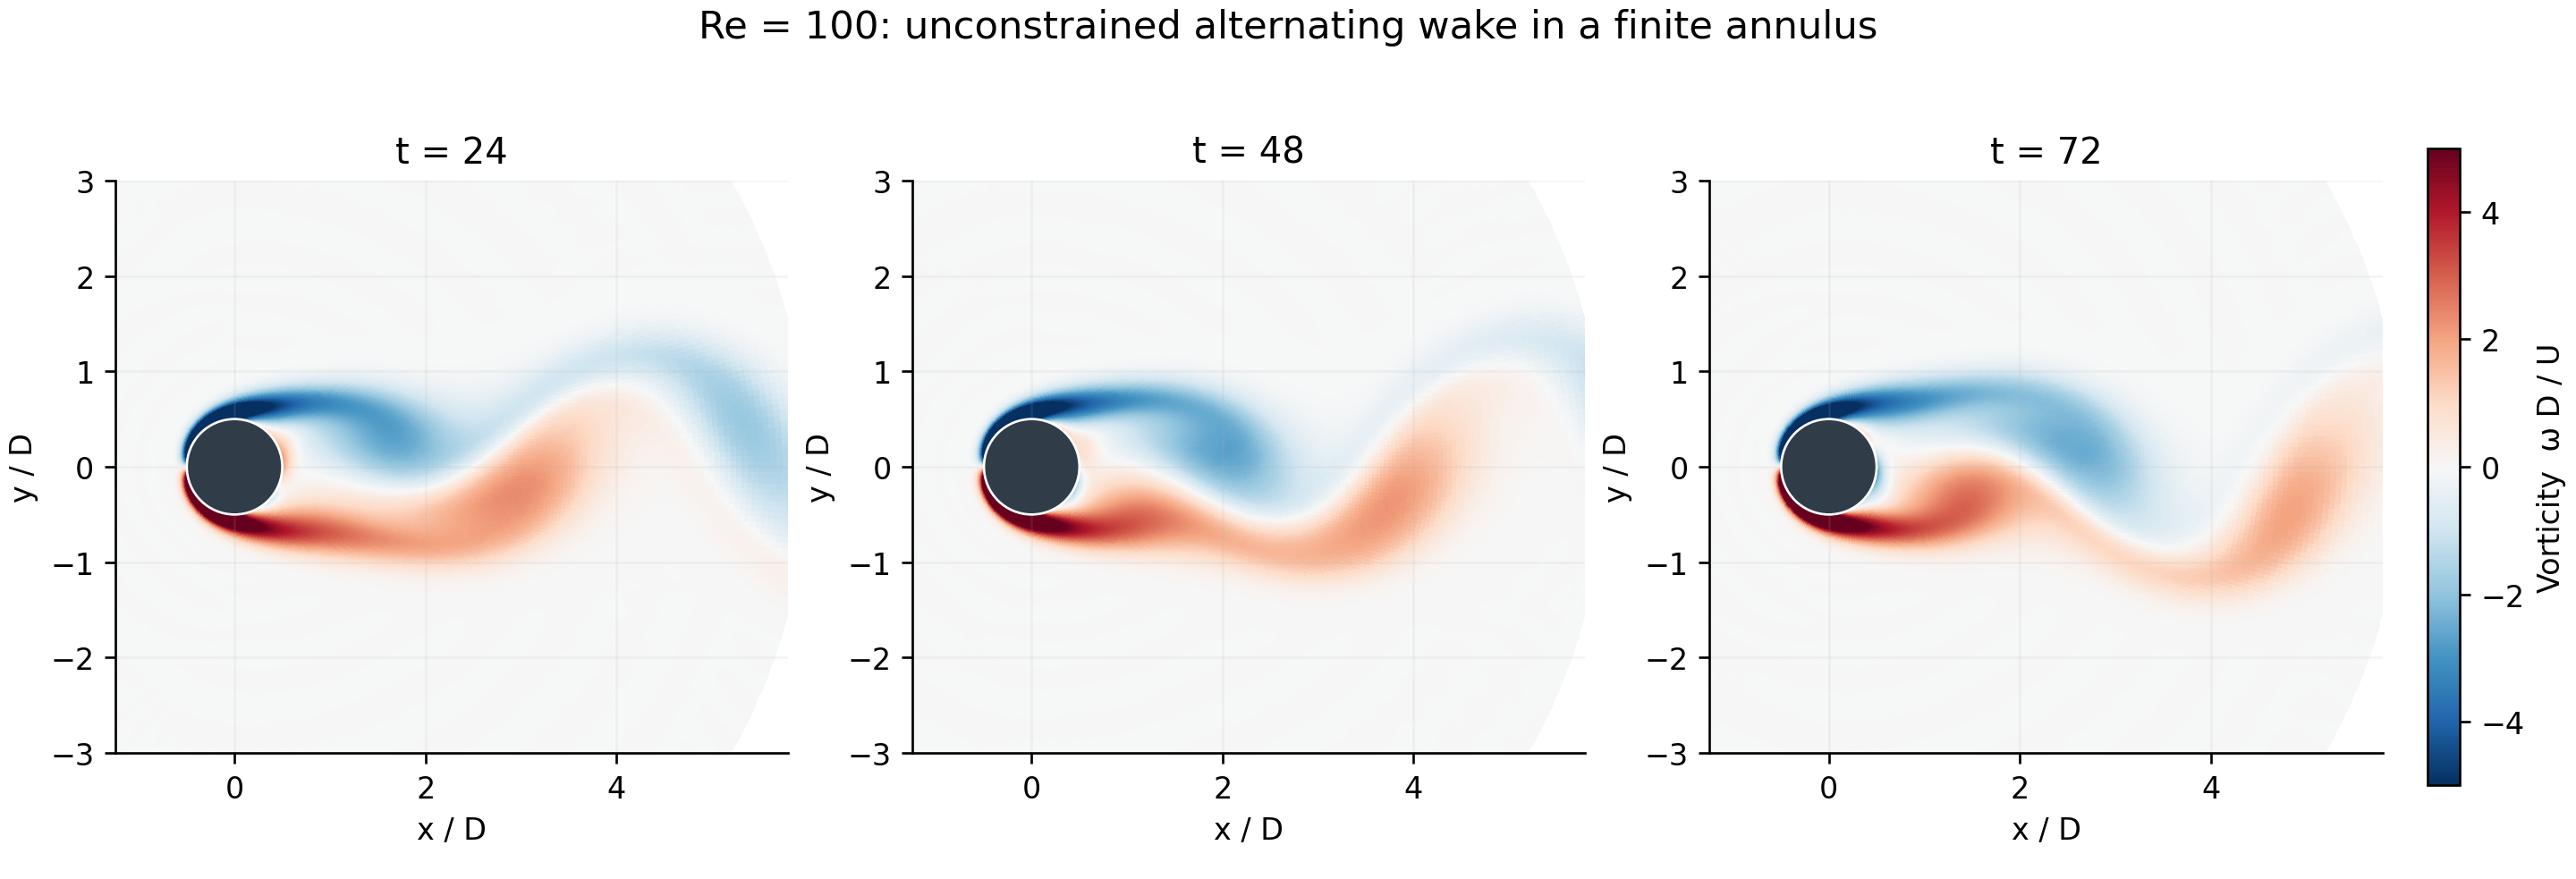
\includegraphics[width=\linewidth]{figures/finite_annulus_vorticity.png}
\caption{Vorticity at $t=24$, $48$, and $72$ for one qualified RFM41 trajectory, without imposed reflection symmetry. The common color scale covers a local view of the annulus; the outer radius is 6.}
\label{fig:annulus-wake}
\end{figure}

\begin{figure}[tbp]
\centering
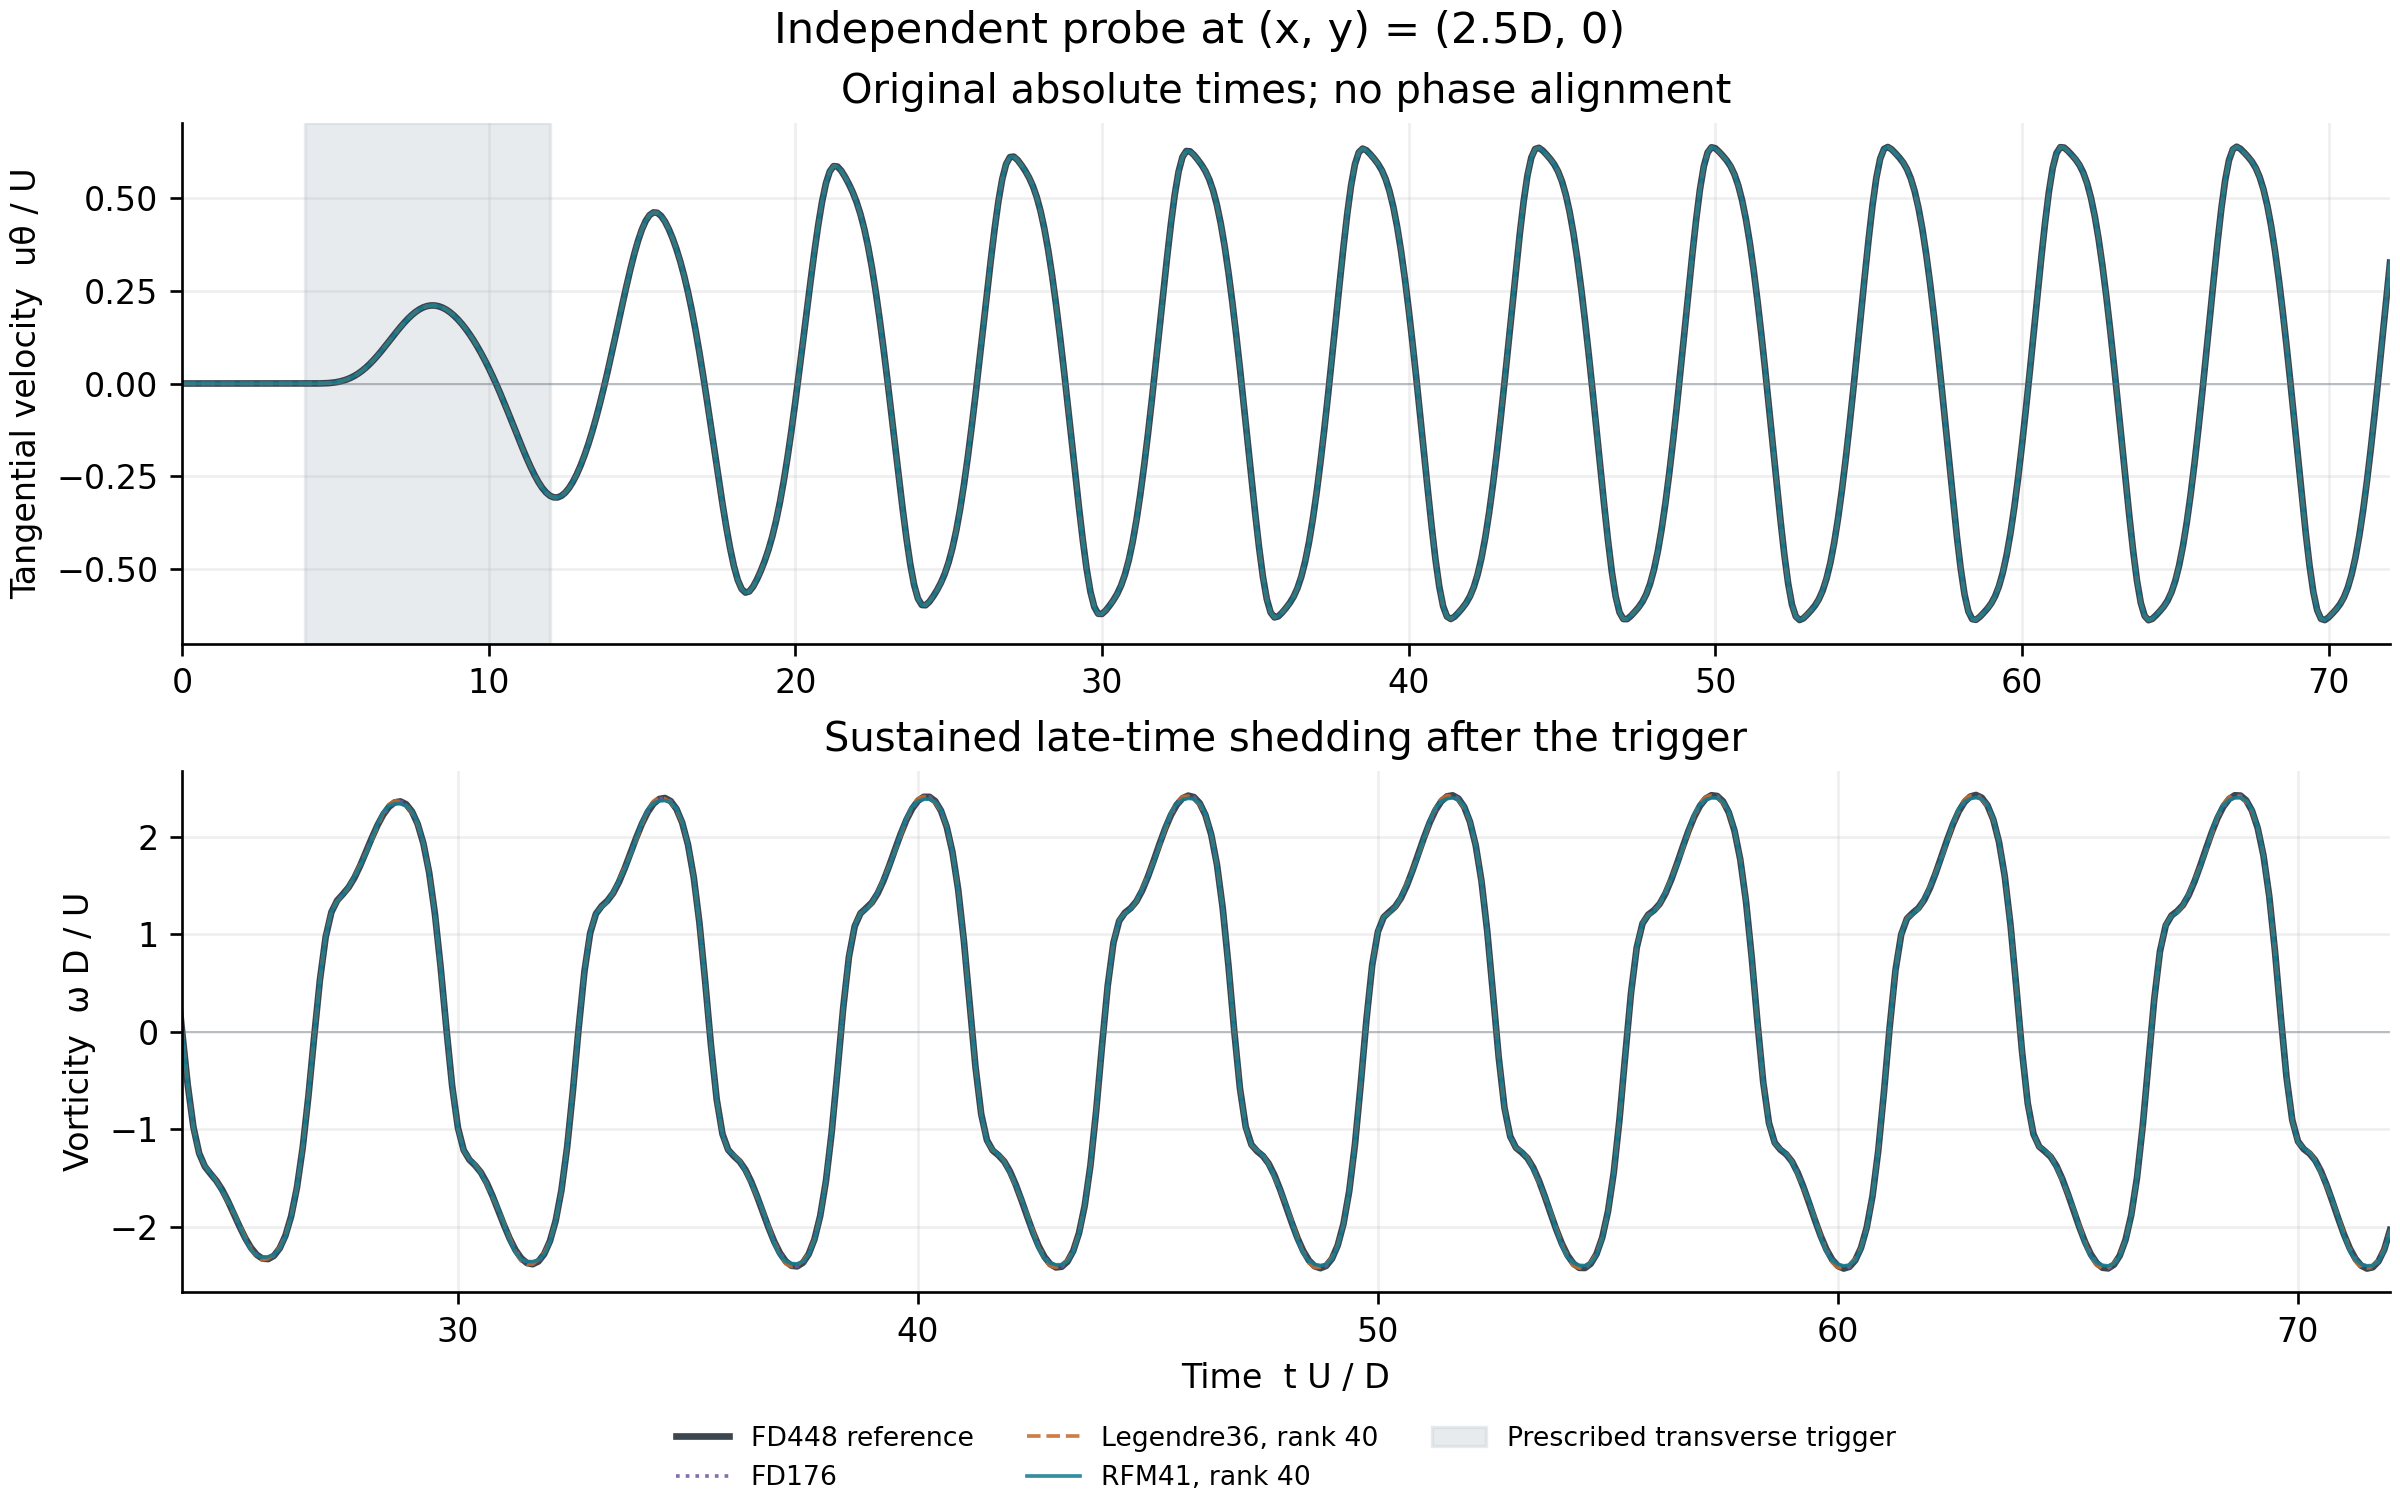
\includegraphics[width=0.88\linewidth]{figures/unshifted_wake_probes.png}
\caption{Unshifted probe histories at $x=2.5D$, $y=0$. Alternating shedding persists after the triggering pulse. RFM41 and FD176 are qualified GPU trajectories, Legendre36 is its corresponding CPU qualification, and FD448 is the reference.}
\label{fig:wake-probes}
\end{figure}

\begin{table}[tbp]
\centering\small
\caption{Recorded nonlinear evaluations for the two piecewise schedules. Both switch at $t=8$ and end at $T=72$.}
\label{tab:workload}
\begin{tabularx}{\linewidth}{@{}Xrrr@{}}
\toprule
Step-rate schedule & Constant step & Piecewise & Reduction \\
\midrule
$128\to112$ & 9,215 & 8,191 & 1,024 ($11.11\%$) \\
$152\to136$ & 10,943 & 9,919 & 1,024 ($9.36\%$) \\
\bottomrule
\end{tabularx}
\end{table}

The counts in Table~\ref{tab:workload} are read from runtime metadata rather than inferred from a nominal order label. Over the remaining 64 time units, reducing the step rate by 16 removes 1,024 steps; the recorded nonlinear counters differ by exactly the same amount. This saving applies to both RFM and Legendre. Reducing retained radial rank does not reduce $q$ or the angular FFT length in these experiments, and therefore does not additionally remove FFTs from each nonlinear evaluation. The work count is an algorithmic saving, while its conversion into elapsed time depends on preparation, linear algebra, observation, and runtime costs.

\section{Additional ablations, error decomposition, and switch sensitivity}
\label{sec:review-experiments}

This section reports 20 new CPU trajectories for the revision: 16 ablation/control runs and four delayed-switch runs. The original 78 GPU qualification records remain frozen. The additional comparisons use the existing two references and physical checkpoints; passing their field tests does not automatically confer promotion under the full probe and GPU-implementation protocol. Concurrent CPU durations are excluded from speed rankings.

\subsection{Additional ablation of frequency jitter and nonzero-mode layers}
\label{sec:review-ablation}
We fixed two configurations,
$(m,K,q,\Delta t^{-1})=(37,72,66,128)$ and $(41,80,76,152)$,
before executing a two-by-two ablation: registered random paired-frequency
jitter $\xi_j\sim U[0.2,0.8]$ versus fixed midpoints $\xi_j=0.5$, and six
nonzero-mode analytic outer-layer features present versus absent.
The random cells use the five registered seeds (7331, 7687, 8011, 8353, 9041).
Each deterministic cell has one unique trajectory; unused seeds are not counted
as replicates. All cells retain the same 24 mean-mode functions, six mean-mode
layers, quadrature, and time step. Adapter checks confirm bitwise equality of
the mean-mode discretization arrays and implicit operators across the four cells.

We computed 16 new CPU trajectories to $T=72$: 14 ablation trajectories and
two enriched-random CPU controls. Ten frozen enriched-random GPU trajectories
were reused and independently rescored. Every trajectory was evaluated at the
same 19 physical checkpoints on three grids against both fine FD references,
using velocity and vorticity errors over the full domain and $r\leq2.5$.
All four errors must be at most 0.5\%.
Table~\ref{tab:review-ablation} gives maxima over seeds, times, grids, and references.
All 16 CPU runs completed without numerical failure; the 12 trajectories without
nonzero-mode layers failed the accuracy gate. The two CPU controls differ from
the archived GPU fields by less than $2.0\times10^{-10}$ in the worst field metric.

\begin{table}[htbp]
\centering\small
\caption{Additional CPU accuracy ablation. Errors are percentages. Pass counts
exclude the two separate CPU controls. Random rows report the worst of five
seeds; midpoint rows contain one deterministic configuration.}
\label{tab:review-ablation}
\begin{tabular}{lrrrrrr}
\hline
Configuration & Rank & $e_u$ & $e_\omega$ & $e_{u,\mathrm{near}}$ & $e_{\omega,\mathrm{near}}$ & Pass \\
\hline
Mid, Random+layer & 39 & 0.0294 & 0.4096 & 0.0251 & 0.2100 & 5/5 \\
Mid, Midpoint+layer & 39 & 0.0293 & 0.4092 & 0.0249 & 0.2097 & 1/1 \\
Mid, Random/no layer & 34 & 19.4054 & 73.8980 & 26.4854 & 48.6306 & 0/5 \\
Mid, Midpoint/no layer & 34 & 19.3644 & 73.7836 & 26.4397 & 48.5825 & 0/1 \\
High, Random+layer & 40 & 0.0182 & 0.3319 & 0.0148 & 0.1799 & 5/5 \\
High, Midpoint+layer & 40 & 0.0181 & 0.3312 & 0.0147 & 0.1794 & 1/1 \\
High, Random/no layer & 35 & 18.7540 & 72.0115 & 25.7262 & 47.7640 & 0/5 \\
High, Midpoint/no layer & 35 & 18.7060 & 71.8705 & 25.6678 & 47.6945 & 0/1 \\
\hline
\end{tabular}
\end{table}

Both midpoint-plus-layer configurations pass, with errors comparable to the
random enriched cells. These data therefore do not establish randomness as
necessary for the observed accuracy. With raw $m$ and the SVD cutoff fixed,
removing the nonzero-mode layers reduces retained rank from 39/40 to 34/35 and
produces large velocity and vorticity errors; the mean rank remains 30.
The compact configurations depend strongly on analytic outer-layer enrichment,
but this design does not separate enrichment geometry from the increased
effective dimension. It is not an equal-rank enrichment ablation, and only one
deterministic frequency design was tested. All four error maxima for both
deterministic no-layer configurations occur at $T=72$. Their maximum vorticity
errors for $t\leq16$ are 2.820\% and 2.592\%, growing to 73.784\% and 71.871\%
at later times. The large errors therefore are not solely a consequence of a
near-zero startup reference field; the mechanism of error amplification is
not established by these data. A subsequent construction-only check increased raw $m$ to
41, 45, 49, 53, 57, and 61 while retaining bandwidth 62, quadrature, and the
SVD cutoff. Both resolutions produced ranks 35, 35, 36, 36, 36, and 36,
respectively, never recovering rank 39 or 40. We therefore did not add a
purported equal-rank $T=72$ control or tune the bandwidth/cutoff after failure.
Concurrent CPU elapsed times are
diagnostic only: they provide neither isolated timing nor new GPU speedup
evidence, and do not extend the original 78 GPU qualification trajectories.

\subsection{Matched-time radial and angular error diagnostics}
\label{sec:review-profiles}

The maximum errors in the qualification tables need not occur at the same time, grid, or reference. We therefore reanalyse the hash-bound CPU controls corresponding to the qualified high-resolution RFM41 (seed 7331), Legendre36, and FD184 trajectories. The first two use the original $t_s=8$ schedule and retain the same nonzero-mode rank 40. The uniform RFM41 and Legendre36 controls are also included in the machine-readable results. Both existing FD448/$K=144$ references are reconstructed: \texttt{angular\_fine} uses rate 384 and \texttt{time\_fine} rate 512. No reference or candidate is integrated for this analysis. All 19 physical times are retained; the figures show the common times $8,24,48,72$ against \texttt{time\_fine}. There is no phase alignment.

Let $e_f$ be the velocity-vector or scalar-vorticity error and let $\langle\cdot\rangle_\theta$ denote the angular mean. For the existing layer144 radial nodes and physical-area weights $w_i$, define
\begin{equation}
R_f^2=\frac{\sum_i w_i\langle|f_{\rm ref}(r_i,\cdot)|^2\rangle_\theta}{\sum_i w_i},
 \qquad P_f(r_i)=\frac{\langle|e_f(r_i,\cdot)|^2\rangle_\theta^{1/2}}{R_f}.
\label{eq:review-profile-norm}
\end{equation}

This normalization avoids dividing by a locally vanishing field. For real fields represented by nonnegative Fourier modes, the angular error contribution is
\begin{equation}
Q_{f,k}=\left(\frac{c_k\sum_i w_i|\widehat e_{f,k}(r_i)|^2}
 {\sum_i w_i\langle|f_{\rm ref}(r_i,\cdot)|^2\rangle_\theta}\right)^{1/2},
 \qquad c_0=1,\quad c_k=2\;(k>0).
\label{eq:review-modal-error}
\end{equation}

For velocity, squared component magnitudes are summed in the polar representation $(u_r,u_\theta)$. The integrated vector-error energy is invariant under the pointwise orthogonal change to Cartesian components, but its allocation among angular modes depends on that representation; the displayed velocity spectrum is therefore a polar-component spectrum. Hence the weighted mean of $P_f^2$ and the sum of $Q_{f,k}^2$ both give the squared relative field error. The exact angular Parseval calculation agrees with the original layer144 physical-grid score to $2.13\times10^{-17}$ in 380 checks. Modes above the candidate cutoff $K=80$ contain the common unresolved reference tail, not additional candidate degrees of freedom.

\begin{figure}[htbp]
\centering
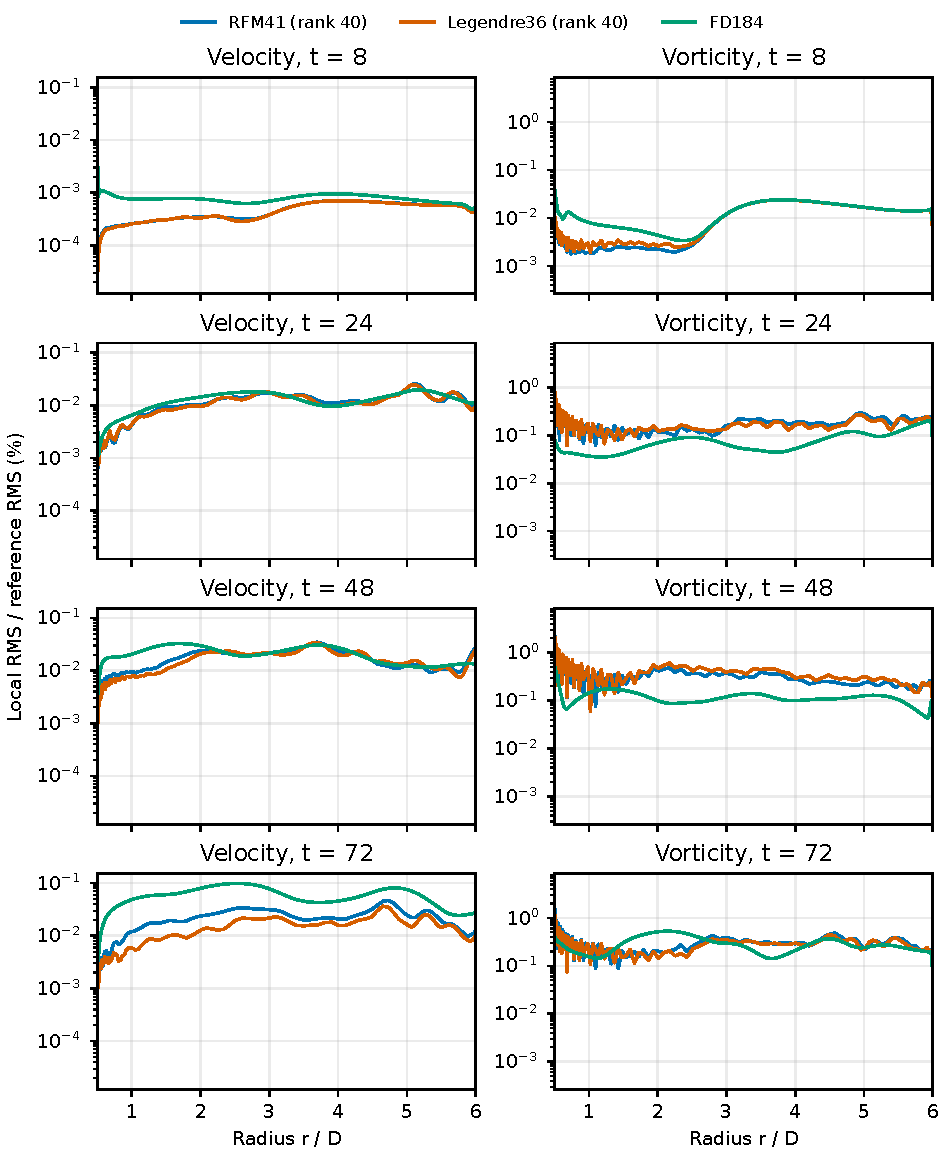
\includegraphics[width=\linewidth]{figures/review_radial_errors.pdf}
\caption{Matched-time radial error profiles $100P_f$ against the existing time-fine reference. RFM41 uses seed 7331. Galerkin curves use $t_s=8$; FD184 retains its qualified schedule. Curves share the same reference and times within each panel. The plotted quantity is a local angular RMS normalized by a global reference RMS, rather than a pointwise relative error.}
\label{fig:review-radial-errors}
\end{figure}

\begin{figure}[htbp]
\centering
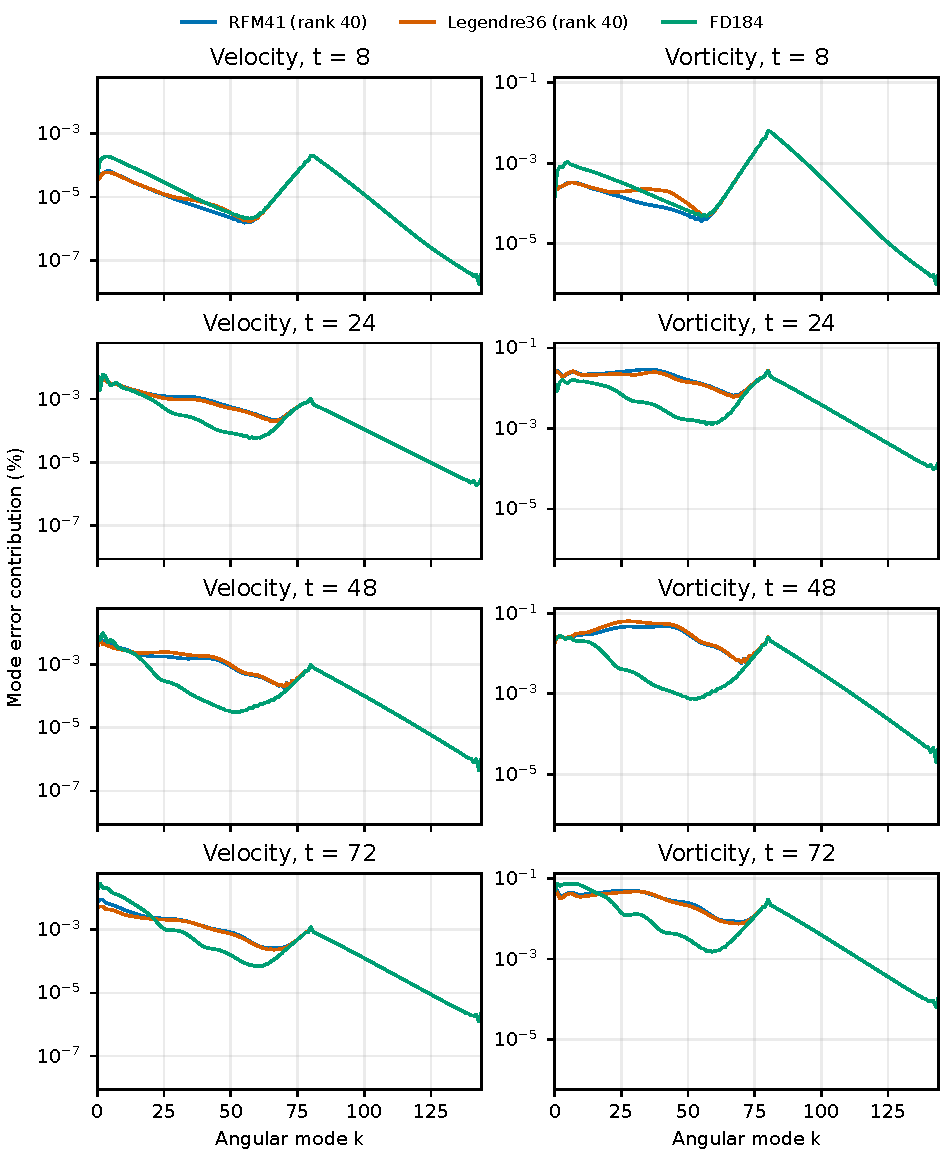
\includegraphics[width=\linewidth]{figures/review_angular_errors.pdf}
\caption{Angular error contributions $100Q_{f,k}$ for the same trajectories and times as Figure~\ref{fig:review-radial-errors}. Contributions combine in quadrature; they are not independently normalized modewise errors. The common tail above mode 80 reflects the finer reference spectrum.}
\label{fig:review-angular-errors}
\end{figure}

The original maxima are not a simultaneous ranking. For this RFM seed, the full-domain velocity and vorticity maxima occur at $t=72$ and $60$; the corresponding Legendre maxima occur at $60$ and $54$. In contrast, at the same $t=48$ and on layer144, RFM41, Legendre36, and FD184 have velocity errors $0.01886\%$, $0.01842\%$, and $0.02053\%$, but vorticity errors $0.29438\%$, $0.35509\%$, and $0.11317\%$. Thus even a simultaneous velocity ranking does not determine the vorticity ranking. Curl depends on first derivatives of velocity; an $L^2$ velocity comparison alone does not control their error. This observation is consistent with the measured spectra: at $t=72$, modes $k\le8$ contain $84.24\%$ of FD184's squared velocity-error norm, whereas modes $25\le k\le80$ contain $47.72\%$ of RFM41's squared vorticity-error norm, compared with $5.45\%$ for FD184.

The radial localization also requires qualification. At $t=72$, $61.14\%$ of RFM41's squared vorticity-error norm lies at $r\ge4$, but only $1.37\%$ lies at $r\ge5.9$. The observed error is therefore not confined to the narrow outermost layer. These diagnostics localize error in the full evolved solutions. They do not identify a causal benefit of the layer basis, or separate radial approximation, time discretization, boundary treatment, and reference uncertainty. The accompanying controlled ablation addresses basis attribution; the present figures alone do not.

\subsection{A CPU sensitivity experiment at $t_s=12$}
\label{sec:review-switch}

Revision 3 added four actual CPU trajectories through $T=72$: RFM37 and Legendre35 at rates $128\to112$, and RFM41 and Legendre36 at $152\to136$, switching at $t_s=12$ instead of 8. RFM uses seed 7331; the deterministic controls retain their original configurations. The generic CPU phase clock already accepts an explicit switch time. Its default observation list contains the old $t_s=8$ bridge instants, so this driver supplies the 19 common physical times explicitly. The underlying solver and archived data are unchanged. Four workers each use one BLAS thread; their elapsed times are not isolated performance evidence. Existing uniform and $t_s=8$ CPU controls are reused, rather than rerun or counted as new experiments.

All four new trajectories match the corresponding uniform CPU states exactly at the saved times $t\le12$. Both full-domain and near-field velocity and vorticity pass the $0.5\%$ threshold on all three grids against both frozen references; the per-cell triangle safeguard relative to the matching uniform control also passes, and alternating probe signs persist. Table~\ref{tab:review-switch12} reports full-domain field maxima separately from the worst safeguard across all four metrics. These are one-seed sensitivity results, not a new five-seed GPU qualification.

\begin{table}[htbp]
\centering\small
\begin{tabular}{llrrrr}
\hline
Configuration & Schedule & $E_u$ (\%) & $E_\omega$ (\%) & Guard (\%) & $N_{\rm nl}$\\
\hline
RFM37 & Uniform & 0.029428 & 0.409349 & 0.409349 & 9215\\
 & $t_s=8$ & 0.044672 & 0.431680 & 0.478647 & 8191\\
 & $t_s=12$ & 0.043821 & 0.429910 & 0.474465 & 8255\\
Legendre35 & Uniform & 0.026763 & 0.442065 & 0.442065 & 9215\\
 & $t_s=8$ & 0.041043 & 0.456649 & 0.497730 & 8191\\
 & $t_s=12$ & 0.040211 & 0.455435 & 0.493773 & 8255\\
RFM41 & Uniform & 0.018192 & 0.331380 & 0.331380 & 10943\\
 & $t_s=8$ & 0.025948 & 0.339890 & 0.368159 & 9919\\
 & $t_s=12$ & 0.025496 & 0.339258 & 0.365822 & 9983\\
Legendre36 & Uniform & 0.016132 & 0.362049 & 0.362049 & 10943\\
 & $t_s=8$ & 0.019717 & 0.366338 & 0.394046 & 9919\\
 & $t_s=12$ & 0.019410 & 0.365962 & 0.391767 & 9983\\
\hline
\end{tabular}
\caption{CPU switch-time sensitivity at the frozen spatial configurations. Errors maximize over two references, three grids, and 19 common times; each metric has its own argmax. The guard also includes the near-field metrics. RFM rows use seed 7331 and therefore need not equal the earlier five-seed maxima. $N_{\rm nl}$ counts actual nonlinear evaluations; the number of marching FFT batches is $2N_{\rm nl}$. No GPU trajectory is available for $t_s=12$, so no CPU--GPU bound is assigned to those rows.}
\label{tab:review-switch12}
\end{table}

Moving the switch from 8 to 12 adds 64 nonlinear evaluations and 128 FFT batches in every configuration. It removes 960 evaluations relative to the uniform schedules: $10.418\%$ at the middle scale and $8.773\%$ at the high scale, versus $11.112\%$ and $9.358\%$ for switching at 8. The measured error decrease is modest: for RFM37 the velocity maximum decreases by $0.000851$ percentage points and the vorticity maximum by $0.001771$ percentage points. The closest new safeguard is $0.493773\%$ for Legendre35. The later switch therefore trades a small increase in work for a small accuracy margin on this case; no isolated speed ranking follows.

The triggering transverse pulse terminates at $t=12$. Its $\sin^4$ profile is $C^3$ at that junction, with a possible fourth-derivative jump. The local Taylor consistency calculation for the bridge must respect the available one-sided regularity there. This experiment is a switch-time sensitivity test, not evidence that a smooth-transient order reduction has been removed. No timestep-refinement series is supplied to estimate an observed order. Separately, the archived $10^{-5}$ implementation gate compares CPU/GPU or CPU operator implementations of the \emph{same} discrete schedule. It is not a tolerance for changing from uniform to mixed timesteps; that change is assessed by the physical errors and the $0.5\%$ safeguard. In the quoted middle-scale RFM comparison, the velocity maxima $0.029428\%$ and $0.044672\%$ differ by $0.015244$ percentage points (about $51.8\%$ relatively), and both happen to occur at $t=72$. This relative increase alone establishes neither a transient-splitting mechanism nor order reduction.

\paragraph{A norm reduction is not a causal error budget.}
For the middle RFM velocity maxima, postponing the switch recovers approximately $5.584\%$ of the increase relative to the uniform schedule. This is the arithmetic ratio $(E_8-E_{12})/(E_8-E_U)$; it does not isolate a bridge-local error. The intervention simultaneously changes four time units of fine versus coarse integration, the bridge time and state, and the subsequent error history. Moreover, $t=8$ is inside the analytic pulse, not a nonsmooth forcing junction.

The saved fields make the nonadditivity explicit. Let $e_8=u_8-u_{\rm ref}$, $e_{12}=u_{12}-u_{\rm ref}$ and $\delta=e_8-e_{12}$, with a common physical-area inner product divided by $\|u_{\rm ref}\|^2$. Then
\begin{equation}
 \|e_8\|_{\rm ref}^2=\|e_{12}\|_{\rm ref}^2+
 2\langle e_{12},\delta\rangle_{\rm ref}+\|\delta\|_{\rm ref}^2.
 \label{eq:review-switch-attribution}
\end{equation}
At $t=72$ on layer144 against the time-fine reference, for RFM37 seed7331 these four terms are $1.9956194141\times10^{-7}$, $1.9202943907\times10^{-7}$, $7.4475738974\times10^{-9}$ and $8.4928450335\times10^{-11}$, respectively. They are squared relative errors, without percent scaling. The unrounded identity residual is $2.04\times10^{-22}$; the cross term accounts for about $98.87\%$ of the squared-norm difference. This deterministic identity illustrates why neither the $5.6\%$ recovery nor its $94.4\%$ complement is an independent physical error component. A causal bridge/coarse-step split would need separately controlled interventions and a timestep-refinement study.



\FloatBarrier


\section{Operator performance and the cost of a complete solve}
\label{sec:performance-results}

\subsection{FFT fusion: a local improvement with first-use overhead}

\begin{table}[tbp]
\centering\small
\caption{Fixed-state CUDA graph event measurements in microseconds per nonlinear evaluation. Each configuration uses nine samples of 64 evaluations. Ratios refer only to this operator measurement.}
\label{tab:fusion-events}
\begin{tabularx}{\linewidth}{@{}Xrrr@{}}
\toprule
Configuration & Original cuFFT & Fused & Local ratio \\
\midrule
Galerkin $N=225$, $q=66$ & 42.12 & 22.64 & 1.86 \\
Galerkin $N=243$, $q=76$ & 40.32 & 25.48 & 1.58 \\
FD176, $N=243$ & 85.13 & 61.00 & 1.40 \\
FD184, $N=243$ & 90.35 & 69.38 & 1.30 \\
\bottomrule
\end{tabularx}
\end{table}

Table~\ref{tab:fusion-events} measures repeated evaluations on a fixed state with hot input arrays. It excludes model construction, compilation, module loading, FFT planning, and physical trajectory advancement. The fused implementation improves all four measured nonlinear operators. Its advantage is largest for the smaller Galerkin batch; the table does not establish a general advantage over cuFFT on arbitrary transforms or hardware. The comparison is between complete nonlinear pipelines with the same output definition, rather than a single custom FFT and an unrelated library call.

The eight subsequent $T=9$ trajectories all passed the reference and implementation tests. Relative to the same warp-observer cuFFT path, the maximum field difference was approximately $1.78\times10^{-9}$; the maximum difference from the independent CPU trajectory was approximately $2.26\times10^{-7}$. Marching was $9\%$--$17\%$ faster. Nevertheless the first complete solve was $23\%$--$69\%$ slower. Compilation and module loading increased by approximately $0.25$--$0.62$~s, while marching saved only $0.017$--$0.030$~s. Figure~\ref{fig:fusion-cost} makes this reversal visible without adding overlapping timing categories.

\begin{figure}[tbp]
\centering
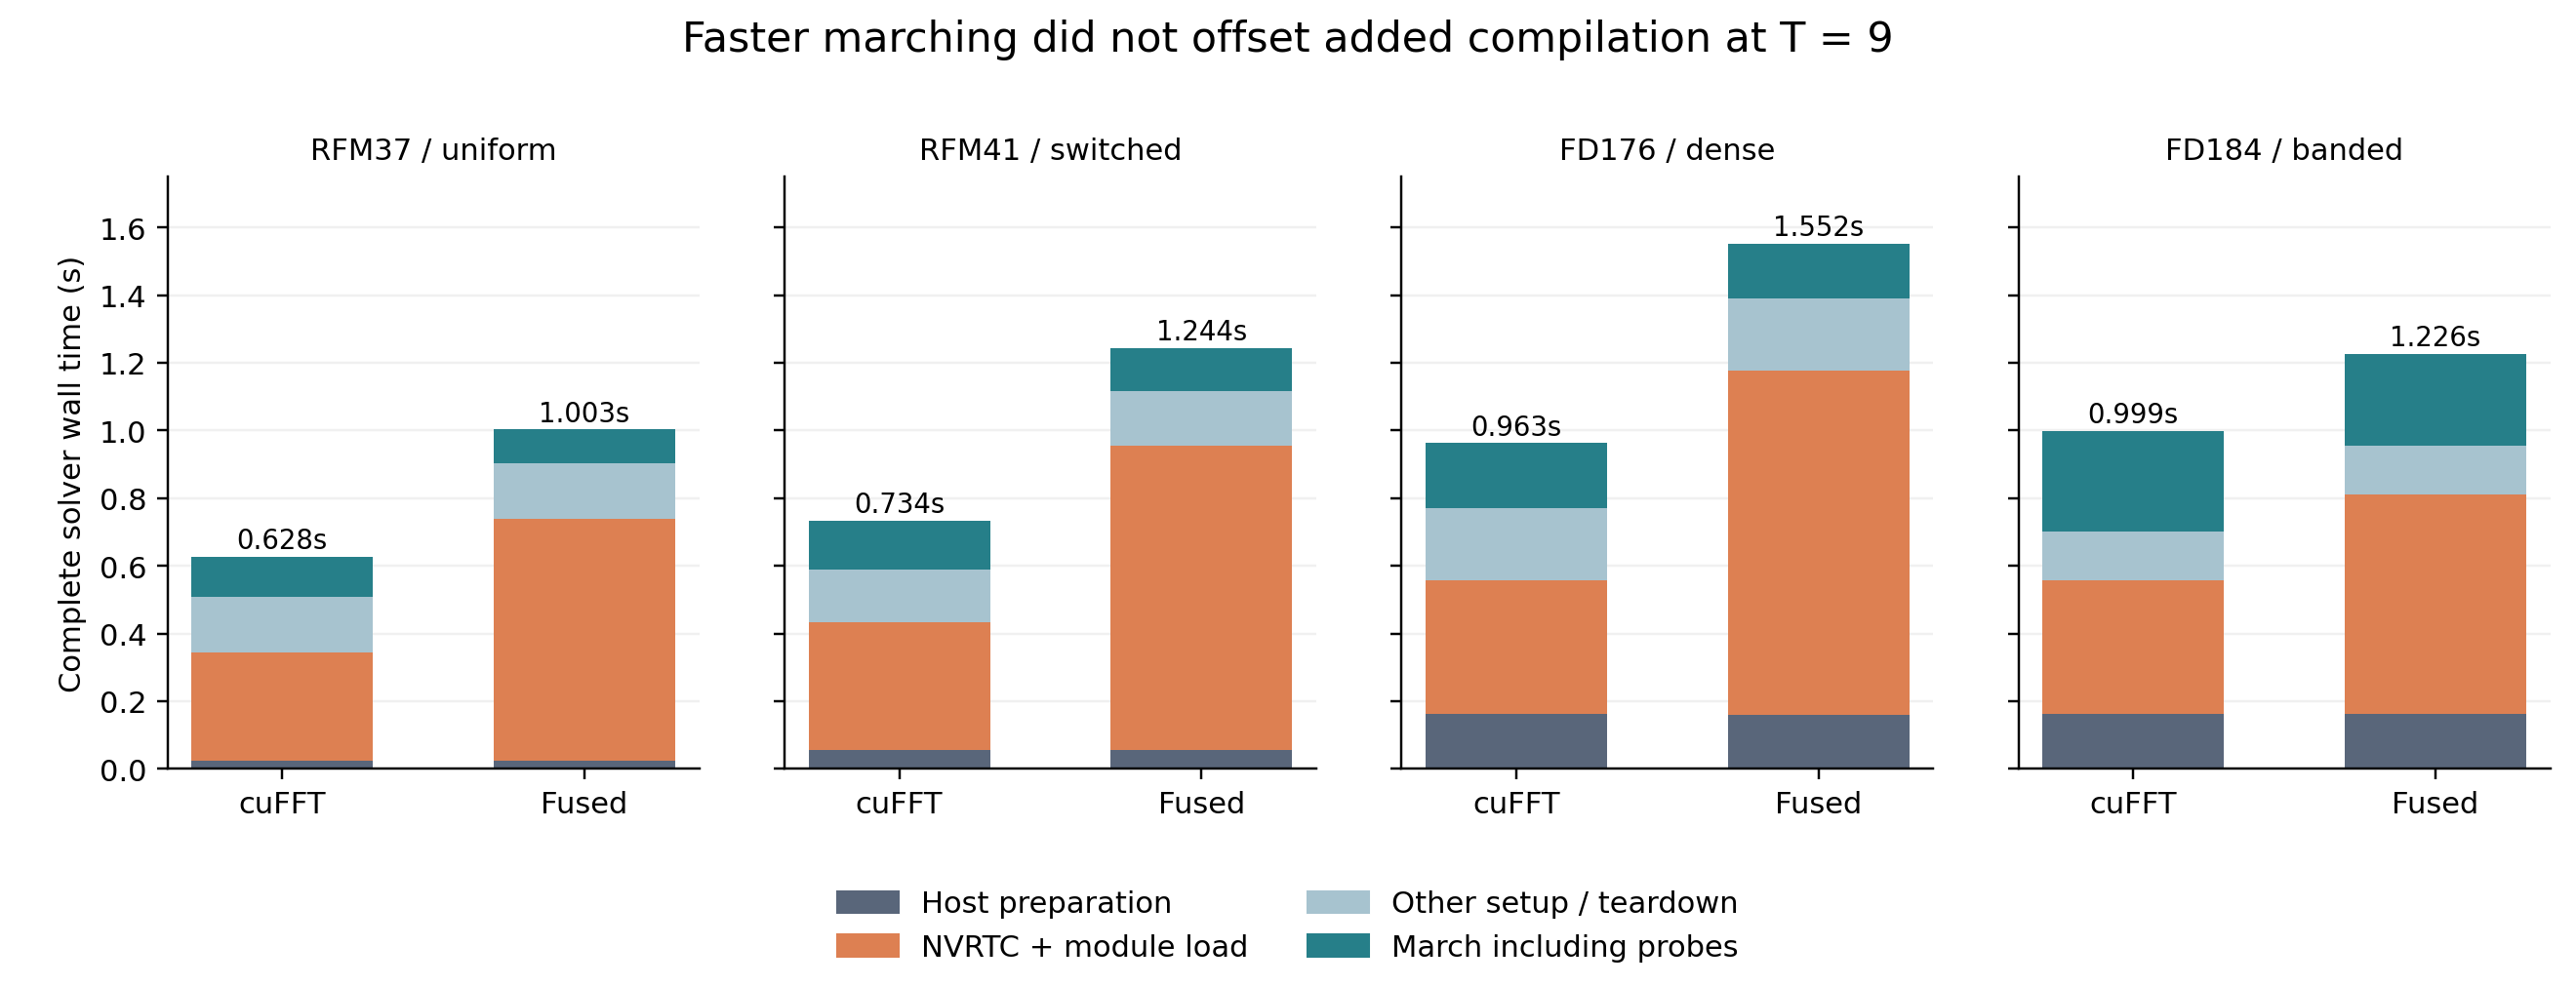
\includegraphics[width=\linewidth]{figures/t9_fusion_cost_breakdown.png}
\caption{Cost decomposition of the sequential $T=9$ fusion diagnostics. Compilation and loading are separated from the remaining runtime initialization. These diagnostic measurements identify first-use costs; they do not provide the missing final $T=72$ ranking.}
\label{fig:fusion-cost}
\end{figure}

Caching changes this tradeoff but did not remove the admission requirement. In the later strict-hit diagnostics, all four complete solver clocks improved, whereas only two of the four fresh-process comparisons improved. The candidate therefore failed its registered promotion rule and was excluded from the final $T=72$ cohort. This is an engineering selection failure, not a failure of its short-trajectory numerical tests. Extrapolating the local ratio to a long trajectory would neglect both overhead and changes in the distribution of work.

\subsection{Observation kernels and common implementation benefits}

Warp-based reduction improves a different part of the pipeline. Fixed-state probe-only nodes decrease from approximately $117$--$147\,\mu$s to $6$--$7\,\mu$s for the tested Galerkin paths, from $727.5$ to $26.2\,\mu$s for FD176, and from $760.3$ to $28.3\,\mu$s for FD184. The resulting local ratios are approximately 19--27. Five full $T=72$ checks preserve the saved states and times bitwise; the changed summation order gives a maximum relative probe difference of $9.26\times10^{-14}$. The operator does not alter the evolution equations.

Because the original FD observation node is more expensive, giving this optimization only to the proposed Galerkin solver would distort the comparison. The final cohort uses the warp observer for all relevant baselines. Multiplying hot-kernel savings by the observation count can suggest where time is spent, but it is not a substitute for the complete paired timing of the modified solver. The local ratio must not be quoted as a 19--27-fold solver speedup.

\subsection{Cache policy, startup, and amortization}

The explicit cache stores PTX compiled from project kernels; it does not store a precomputed solution, spatial matrices, CUDA context, or cuFFT plan. The key binds source, compiler options, target architecture, entry points, compiler identity, and dependency hashes. Under \texttt{strict\_hit}, a missing or corrupt artifact is an error, with no silent compilation fallback. Under \texttt{empty\_first}, each run begins with a new directory and pays for compilation, atomic writing, readback verification, and loading. Driver and operating-system caches remain in their natural state. Thus ``first use'' is an explicit policy, not a claim that the whole machine has been reset to a cold state.

Three stock PTX keys occupy 147,782 bytes. Three fresh-process installations take $2.7292$, $2.6392$, and $2.6487$~s, with a median of $2.6487$~s. Reporting only the roughly $0.93$~s NVRTC stage would omit most of this installation path. If $C$ is the complete installation cost, $H$ a subsequent hit cost, and $F$ a per-solve first-use cost under otherwise matched conditions, the amortized comparison is
\begin{equation}
\label{eq:cache-amortization}
 T_{\rm cache}(n)=C+nH,\qquad T_{\rm first}(n)=nF.
\end{equation}
A crossover requires $F>H$ and $n>C/(F-H)$. The final campaign does not provide an accepted paired estimate of $F-H$, so no measured break-even solve count is reported. The installation covers three keys; the minimum installation cost for a user needing only one key was not measured.

An earlier 50-run high-resolution campaign passed its sampled isolation check and measured median paired fresh-process speedups of 1.293 and 1.301 after import simplification for constant and piecewise RFM, while solver-time ratios stayed near unity. This identifies a startup improvement for that historical configuration. It does not replace a comparison with the stronger Legendre baseline, common warp observer, or explicit cache policies introduced later. Pooling these rows would mix different experimental treatments.

\subsection{A conditional crossover for a longer time schedule}
\label{sec:schedule-amortization}

The historical single-bridge diagnostic records about $\Delta M_0=0.119$~s of marching savings and $\Delta P=0.206$--$0.240$~s of additional preparation. These measurements come from a window marked \texttt{diagnostic\_only}, with external activity, and precede the final configuration set. They cannot supply a measured final speed ratio. They can, however, make the assumptions of a crossover estimate explicit.

Let $N$ count steps of the piecewise candidate, including the unchanged first $N_s=1024$ steps. Its $T=72$ trajectory has $N_0=8192$ steps. If the extra preparation stays constant and the saved marching time grows linearly with only the later work, the modeled candidate-minus-control time is
\begin{equation}
 \Delta T(N)=\Delta P-
       \frac{N-N_s}{N_0-N_s}\Delta M_0,\qquad
 N_* = N_s+(N_0-N_s)\frac{\Delta P}{\Delta M_0}.
 \label{eq:schedule-amortization}
\end{equation}
Substitution gives $N_*\simeq13{,}432$--$15{,}480$ candidate steps. A coarser model that scales the savings with all steps instead gives $N_*=N_0\Delta P/\Delta M_0\simeq14{,}181$--$16{,}522$. Their difference reflects the treatment of startup, not additional measurements. Thus a scale of roughly $1.5\times10^4$ steps is a conditional planning estimate, not an observed threshold. Neither model proves accuracy beyond $T=72$, constant device efficiency, or superiority to a different qualified method. Multiple short solves amortize preparation only when the relevant prepared objects are actually shared; a PTX cache alone does not share spatial matrices or FFT plans. A new longer-horizon qualification and isolated experiment are required to validate a crossover.


\section{Rejected candidates and the limits of local theory}
\label{sec:negative-results}

\subsection{Common phase coordinates and dense output layout}

The common phase-basis prototype improves local linear-algebra diagnostics but, with the existing dense device interface, increases three-phase preparation by about $37\%$--$58\%$. Table~\ref{tab:phase-setup} reports the measured values. Device storage remains $11.69$--$16.30$~MB because dense physical-coordinate operators are still generated. The prototype pays for eigendecomposition and back-transformation of wide right-hand-side blocks instead of remaining in diagonal coordinates throughout the computation.

\begin{table}[tbp]
\centering\small
\caption{Local phase-preparation measurements in milliseconds. These use the prototype's original anchor, not the later geometric-anchor rule.}
\label{tab:phase-setup}
\begin{tabularx}{\linewidth}{@{}Xrrr@{}}
\toprule
Configuration & Original & Triangular solves & Common phase basis \\
\midrule
Mid RFM & 34.27 & 47.41 & 51.96 \\
Mid Legendre & 34.81 & 44.72 & 47.73 \\
High RFM & 38.75 & 56.39 & 61.39 \\
High Legendre & 45.71 & 62.00 & 66.22 \\
\bottomrule
\end{tabularx}
\end{table}

The analytical anchor in Eq.~\eqref{eq:anchor} minimizes a condition-number upper bound. It was not timed as a new production candidate. Better transformed conditioning, fewer factorizations, less stored data, and shorter complete runtime are distinct propositions. A future implementation that keeps state in common coordinates would need corresponding reconstruction, lifting, projection, and observation operators, followed by a new floating-point and trajectory qualification. The existing prototype does not test that architecture.

\subsection{Energy structure does not guarantee coarse-step accuracy}

The Lamb--BDF2 candidate freezes an extrapolated vorticity field and solves the resulting velocity system iteratively. Appendix~\ref{sec:app-lamb} derives the discrete skew-symmetry and fixed-step energy identity, including boundary and algebraic-residual work. These properties concern the stated discrete update and norms. They do not eliminate the error introduced by extrapolating vorticity or establish accuracy at an arbitrarily large step.

At $T=16$ and step rate 128, the worst vorticity errors are $0.364950\%$ for RFM37 and $0.364784\%$ for Legendre37, satisfying the $0.5\%$ field criterion. At rate 64 they rise to approximately $161.024\%$ and $161.664\%$. The first saved failing state occurs at $t=4$, before the transverse pulse begins. At the recorded checkpoints the original-equation residuals remain at most $7.590\times10^{-10}$, and work-corrected energy defects remain at most $2.25\times10^{-15}$. A tightly solved linear system and a closed energy identity can therefore coexist with an inaccurate flow trajectory.

The qualifying rate-128 candidate requires approximately $5.03$ times as many one-dimensional FFTs as the explicit control in the same space. This count includes products needed by the iteration and residual checks; halving nominal time steps alone would hide that work. The rate-64 variants also require more transforms and fail accuracy. The branch was consequently rejected before a $T=72$ GPU comparison.

\subsection{Skipping nonlinear evaluations and changing graph schedules}

Evaluating the nonlinear term on alternate steps gives an appealing nominal reduction. Scalar tests of the corresponding history extrapolation show observed convergence orders of $1.998$--$2.016$. However, corrected Navier--Stokes pilots that activate this strategy after $t=8$ overflow near $t=9.508$ and $9.559$, while their ordinary controls complete. The failed trajectories do not supply valid accuracy or timing results. This experiment illustrates why local consistency and scalar stability probes are screening tools rather than guarantees for the driven, mode-coupled discretization.

Two implementation experiments were numerically successful but did not meet performance-selection criteria. Alternating the two existing spectral-history buffers preserves eight short paired trajectories bitwise but gives inconsistent marching changes of $-0.030$ and $+0.018$~ms in the graph-enabled pair summaries. Changing graph chunk length from 24 to 48, 64, or 128 steps preserves 36 full trajectories bitwise. Although 48 steps halves the scheduled graph launches, no alternative simultaneously meets the registered marching, solver, and fresh-process improvement criteria. These diagnostics lack full external-load isolation and do not establish small stable speed differences. The 24-step graph schedule is retained.

\section{Disposition of the final timing experiment}
\label{sec:timing-disposition}

The final design registers 160 slots across five paired blocks, two cache policies, and the qualified methods. RFM seeds are assigned by block; deterministic methods remain fixed. Both the complete solver clock and the fresh-process clock are needed for a practical result. The latter includes the declared supervisor and process-start costs. Every window must finish its prescribed sequence, satisfy numerical checks, and pass sampled isolation; failed slots are not replaced selectively with cleaner runs.

\begin{table}[tbp]
\centering\small
\caption{Final timing attempts and admissible interpretation. None provides an accepted final paired speed ranking.}
\label{tab:timing-status}
\begin{tabularx}{\linewidth}{@{}p{0.22\linewidth}XX@{}}
\toprule
Attempt & Recorded outcome & Consequence \\
\midrule
Original design & Two slots complete; the third has no confirmed timely terminal state & Incomplete paired blocks \\
First recovery & External activity in preflight; zero slots launched & Window rejected before timing \\
Final recovery & 12 attempted; 11 raw successes; terminal publication fails for the twelfth & Completion requirement fails \\
Independent load check & External CPU activity exceeds the registered budget during the final active window & Isolation fails independently \\
Numerical readback & All 12 saved trajectories match their qualification arrays; 148 slots remain unattempted & Numerical evidence retained; no ranking \\
\bottomrule
\end{tabularx}
\end{table}

In the last attempted slot, the solver writes its numerical output and exits with a successful exact-process status, but a subsequent permission error prevents publication of the terminal state. The available record does not identify the original lock holder. A later CPU-only diagnostic reproduces a file-publication failure under a controlled reader configuration, without proving that it caused the earlier event. Separately, the load monitor observes external CPU activity above $0.2$ CPU seconds per ten-second budget interval. Correcting terminal publication alone would therefore not make the recorded batch admissible.

The isolation mechanism uses sampled process identities and preflight GPU observations, not exclusive ownership enforced by the operating system. Very short processes can escape between samples, and coverage of unrelated applications is limited. Those limitations apply even to historical windows that passed the sampled check. For the final window, the recorded violations are sufficient to reject the timing regardless of the additional unobserved activity that might have existed.

No final speedup, confidence interval, or method ranking is constructed from the 11 successful raw records, from qualification durations, or by joining the two earlier slots to a later recovery. The missing high-resolution windows also prevent a claim of stable behavior across resolutions. The result is an unresolved performance ordering, rather than a measured win or loss of RFM against the strongest classical baseline.

\section{Discussion and conclusions}
\label{sec:discussion}

\subsection{What changes on a nonseparable geometry}
\label{sec:geometry-scope}

The annulus supplies more than a convenient test shape. Its metric and boundary conditions are independent of angle, so the implicit operator separates into angular blocks; the nonlinear products still couple modes. The retained radial rank $d$, number $K$ of positive modes, quadrature size $q$, and padded angular size $N$ lead to dense setup costs of order $Kd^3$ for independent modal factorizations. A step contains order $Kd^2$ modal solves, $qdK$ reconstruction and projection work, and $qN\log N$ transform work. These counts suppress fixed channel counts and the separate mean block. They describe the present implementation, not a complexity theorem for RFM in general. Differential normalization of an $n$-column raw feature matrix additionally costs order $qn^2+n^3$ in the dense regime $q\geq n$.

On an angle-dependent mapped boundary, the metric coefficients and boundary lifting generally depend on angle. Multiplication by these coefficients couples Fourier modes even in the implicit linear operator. The scalar mode equations and their separate common-phase bases then cease to be an exact factorization of the full problem. A naive dense solve with $D=O(Kd)$ coupled degrees of freedom would require $O(D^2)$ storage and $O(D^3)$ factorization. This is an avoidable dense-design cost, not a necessary lower bound: sparse local spaces, matrix-free metric products, domain decomposition, and iterative solvers are alternatives. They require a new operator design and qualification; the present GPU measurements do not test them.

The role of conditioning can be stated precisely without claiming that the annular transform removes it. Let $B$ be an SPD reference implicit operator and $A$ a mapped-domain SPD operator on the same discrete space. If the geometry and boundary construction yield constants $0<\alpha\leq\beta$ such that
\begin{equation}
 \alpha x^\top Bx\leq x^\top Ax\leq\beta x^\top Bx
 \quad\hbox{for all }x,
 \label{eq:geometry-equivalence}
\end{equation}
then the Rayleigh quotient gives
\begin{equation}
 \sigma(B^{-1/2}AB^{-1/2})\subset[\alpha,\beta],\qquad
 \kappa_2(B^{-1/2}AB^{-1/2})\leq\beta/\alpha.
 \label{eq:geometry-condition}
\end{equation}
This is a conditional preconditioning bound. We do not establish mesh-independent $\alpha,\beta$ for an arbitrary body. Distorted mappings, narrow gaps, and nonuniform local resolution can degrade them. Boundary-data approximation introduces a separate consistency error that is not controlled by this spectral bound; it need not alter the implicit matrix. Likewise, the identity $K_1=\nu I$ on the retained annular feature space is an exact-arithmetic normalization at the chosen quadrature; it does not bound every modal mass matrix, discarded approximation direction, or floating-point reconstruction error.

Local random features with partitions of unity provide a documented route to complex interfaces, including linear Stokes examples\cite{r20}. That evidence motivates an extension, but does not validate the present unsteady nonlinear solver on such geometries. A credible extension would preserve boundary and divergence constraints, compare retained dimensions and quadrature work with deterministic local spaces, and repeat both velocity/vorticity qualification and complete-cost timing. Accordingly, our compact-space and kernel conclusions are restricted to the specified separable finite annulus.

Pure radial reparameterization should be distinguished from an angle-dependent geometry. For a smooth invertible map $r=\rho(\eta)$, the metric coefficients remain independent of $\theta$. With the same angularly invariant boundary operators, Fourier orthogonality preserves the implicit modal blocks; only the radial matrices and their conditioning change. The $O(Kd^2)$ independent dense-solve cost remains applicable to the current Galerkin design. A map for an eccentric or noncircular body generally introduces angle-dependent coefficients in this representation and couples angular modes. This observation is about the chosen coordinates and operators, not a theorem that every irregular geometry requires a particular iterative algorithm.

If the coupled implicit matrix $A$ and a fixed preconditioner $B$ are SPD and the assumed spectral-equivalence inequality holds, exact-arithmetic PCG gives the standard energy-error bound\cite{r21}
\begin{equation}
 \frac{\|e_j\|_A}{\|e_0\|_A}
 \leq2\left(\frac{\sqrt{\kappa}-1}{\sqrt{\kappa}+1}\right)^j,
 \qquad \kappa=\kappa_2(B^{-1/2}AB^{-1/2})\leq\beta/\alpha.
 \label{eq:geometry-pcg-bound}
\end{equation}
For $\kappa>1$, this supplies a sufficient iteration scale $O(\sqrt{\beta/\alpha}\log(1/\varepsilon))$ for relative energy-error reduction $\varepsilon$; it is not a measured iteration count or a lower bound. The cost also includes applying $A$, solving with $B$, and reductions. The bound does not automatically apply to nonsymmetric discretizations, indefinite systems, or variable/inexact preconditioners. Smooth mapping alone has not established the needed $\alpha,\beta$ for this study. A pseudospectral metric product may use angular FFTs, whereas an assembled sparse coupling or a short Fourier convolution may use other products. Thus neither PCG nor an FFT at every matrix--vector product is mandatory, and the annular timing results cannot predict the new operator balance.



\subsection{Synthesis and conclusions}

The evidence separates numerical design from implementation. The piecewise schedule removes measured nonlinear evaluations and applies equally to RFM and Legendre. Compact qualifying spaces exist in both basis families. The custom fused operator reduces local nonlinear cost, while the warp reduction removes a substantial observation bottleneck shared by Galerkin and FD. Startup simplification and explicit caching affect different terms of the runtime. None of these facts, individually, establishes an end-to-end advantage from random features.

The closest experimentally supported bottleneck is the mismatch between a short GPU workload and its preparation costs. A historical profile assigns about $0.058$~s of a $1.70$~s full solve to host spatial preparation, approximately $3.4\%$. This is a diagnostic for that configuration, not a universal bound, but it provides little motivation for a wholesale language rewrite. Rewriting a measured hot loop can help; replacing high-level orchestration alone does not reduce the number of nonlinear evaluations, library FFTs, or device matrix operations. High-level flow solvers can already combine efficient kernels and numerical libraries~\cite{r14}.

The finite outer boundary is a major limitation. Increasing $R$ from 6 to 8 produces an unshifted maximum vorticity difference of about $50.39\%$ on the common region $r\leq4$, with accumulated phase differences included. This is a sensitivity result between finite-domain simulations, not a rigorous estimate of exact-solution error. It prevents interpreting the present $0.5\%$ qualification as an infinite-domain cylinder benchmark. The current study also does not validate pressure, drag, lift, three-dimensional turbulence, higher Reynolds numbers, or a hardware-independent speed advantage.

Advanced trained PINN methods were not measured under the same complete field, probe, and timing protocol in this phase. Consequently the paper compares a fixed-feature Galerkin discretization with its deterministic and finite-difference controls, without ranking PINN training methods. Earlier cavity and other flow studies do not automatically inherit the final annulus qualification. Broader claims require new case-specific reference and timing evidence.

The added ablation further shows that deterministic midpoint frequencies with the same analytic layers reach the field tolerance at both resolutions; randomness is not necessary for these configurations. Removing the nonzero-mode layers greatly increases error but also decreases retained rank, preventing an equal-dimensional attribution to a feature family alone. The delayed-switch controls and error profiles clarify accuracy tradeoffs without supplying a new speed ranking.

\label{sec:conclusion}
For the specified $\mathrm{Re}=100$ finite-annulus problem, all 78 registered GPU qualification trajectories meet the common velocity and vorticity criteria. The two piecewise schedules reduce nonlinear evaluations by $11.11\%$ and $9.36\%$. Fused FFT pipelines improve local and short-run marching costs but lose on first-use complete cost; the more aggressive nonlinear-update candidates fail accuracy or workload criteria. The final isolated campaign is not accepted, so a stable complete-solve speed advantage over the optimized Legendre and fourth-order spatial FD baselines remains unestablished. The defensible contribution is the explicit mathematical adaptation, kernel implementation, and evidence-based attribution of these distinct effects.

\section*{Data and code availability}

The original NS evidence corresponds to archived revision
\href{https://github.com/LStar404/rfm-navier-stokes-research/tree/6f2b3500964d3d5153b8400018236c4702ef94f8}{\texttt{6f2b350}}, retaining source, protocols, configuration identities, qualification scores, and failed attempts. Appendix~\ref{sec:app-evidence} maps these archived tables and figures to their source records. The repository is publicly accessible; the archived commit and revision inventories identify the corresponding evidence.

The new evidence is stored separately in \path{work/rfm_review_v3/}. The \texttt{ablation/} directory contains 16 CPU ablation/control trajectories, rescoring of ten frozen GPU controls, 12 capacity-construction checks, and coverage verification. The \texttt{profiles\_bridge/} directory contains four delayed-switch CPU trajectories, radial and angular error data, cellwise two-reference scores, and Parseval checks. The \texttt{maintenance/} directory contains the explicit-factory maintenance package and seven tests. Protocols, source hashes, outputs, and analysis scripts accompany the revision without overwriting the frozen evidence. These 20 new CPU trajectories do not increase the original GPU qualification count or establish a new isolated performance result. The previous standalone GPU operator example and its 36 correctness cases remain separately identified. The point-by-point response is provided as \path{response.tex} in the same manuscript project.
